\documentclass[11pt]{article}
\usepackage[T1]{fontenc}
\usepackage{lmodern}
\usepackage[margin=1in]{geometry}
\usepackage{amsmath,amssymb,amsthm,mathtools}
\usepackage{microtype}
\usepackage{needspace}
\usepackage{xcolor}
\usepackage{tikz}
\usetikzlibrary{arrows.meta,positioning}
\definecolor{linkblue}{RGB}{28,65,105}
\usepackage[colorlinks=true,allcolors=linkblue]{hyperref}
\hypersetup{pdftitle={A C1 Counterexample to the Entropy Conjecture},
            pdfauthor={OpenAI}}
\usepackage[nameinlink,noabbrev,capitalise]{cleveref}
\pdftrailerid{}
\newtheorem{theorem}{Theorem}[section]
\newtheorem{lemma}[theorem]{Lemma}
\newtheorem{proposition}[theorem]{Proposition}
\newtheorem{corollary}[theorem]{Corollary}
\theoremstyle{definition}
\newtheorem{definition}[theorem]{Definition}
\theoremstyle{remark}
\newtheorem{remark}[theorem]{Remark}
\newcommand{\C}{\mathbb C}
\newcommand{\R}{\mathbb R}
\newcommand{\Z}{\mathbb Z}
\newcommand{\N}{\mathbb N}
\newcommand{\htop}{h_{\mathrm{top}}}
\newcommand{\id}{\mathrm{id}}
\DeclareMathOperator{\supp}{supp}
\DeclareMathOperator{\pr}{pr}
\title{A \(C^1\) Counterexample to the Entropy Conjecture}
\author{OpenAI}
\date{September 25, 2026}
\begin{document}
\maketitle

\begin{abstract}
We disprove the general \(C^1\) self-map formulation of Shub's entropy
conjecture. We construct a noninvertible \(C^1\) self-map of a compact
smooth manifold without boundary whose topological entropy is zero,
while its action on second real homology has eigenvalue \(2\). Thus the
topological entropy is strictly smaller than the logarithm of the
homological spectral radius.
\end{abstract}

\section{Introduction}\label{sec:introduction}

Let \(M\) be a nonempty compact smooth manifold and let \(f:M\to M\) be
continuous. For a compatible metric \(d\), write
\[
 d_n(x,y)=\max_{0\le j<n}d(f^j(x),f^j(y)),
\]
and let \(s_f(n,\varepsilon)\) be the largest cardinality of a set whose
distinct points satisfy \(d_n(x,y)>\varepsilon\). The topological entropy is
\[
 \htop(f)=\lim_{\varepsilon\downarrow0}
 \limsup_{n\to\infty}\frac1n\log s_f(n,\varepsilon).
\]
It is independent of \(d\). Throughout, homology means singular homology
with real coefficients. The induced map \(f_*\) acts on the finite-dimensional
space
\[
 H_*(M;\R)=\bigoplus_{k=0}^{\dim M}H_k(M;\R),
\]
and \(\rho(f_*)\) denotes its spectral radius.

Shub's entropy conjecture relates orbit complexity to the growth visible
in homology \cite{Shub1974}. Shub's later account explicitly includes
endomorphisms as well as diffeomorphisms and distinguishes the earlier
Lipschitz counterexamples discussed by Pugh from the \(C^1\) question
\cite[Section~2]{Shub2007}.
In the general \(C^1\) self-map formulation recorded by
Saghin and Xia \cite[Conjecture~1]{SaghinXia2010}, it asks whether
\begin{equation}\label{eq:conjecture}
 \htop(f)\ge \log\rho(f_*)
\end{equation}
holds for every \(C^1\) map of a compact smooth manifold without boundary.
Several positive results mark the scope of this question. Manning's
inequality controls the action on \(H_1(M;\R)\) for every continuous
map \cite{Manning1975,Manning1976}. Misiurewicz and Przytycki's
\(C^1\) lower bound concerns topological degree, hence top-dimensional
homology \cite{MisiurewiczPrzytycki1977,Manning1976}. Yomdin proved
\eqref{eq:conjecture} for \(C^\infty\) maps by controlling homological
growth through volume growth \cite{Yomdin1987}. Gromov explains the
regularity estimates and their \(C^\infty\) consequence
\cite[Sections~2.2--2.3]{Gromov1987}.
Among restricted \(C^1\) classes, Saghin and Xia proved the bound for
partially hyperbolic diffeomorphisms with one-dimensional center
\cite[Theorem~1]{SaghinXia2010}; Liao, Viana, and Yang established it
for diffeomorphisms away from homoclinic tangencies
\cite[Theorem~A]{LiaoVianaYang2013}.
None of these statements covers the combination of finite regularity,
noninvertibility, and intermediate-degree homology used below.

\Needspace{8\baselineskip}
\begin{theorem}\label{thm:main}
There are a positive integer \(q\) and a \(C^1\) self-map \(f\) of the
compact smooth manifold
\[
 M=(\R/100\Z)\times(S^2)^{q+1}
\]
such that \(\htop(f)=0\) and \(f_*:H_2(M;\R)\to H_2(M;\R)\) has
eigenvalue \(2\). In particular,
\[
 \htop(f)=0<\log 2\le \log\rho(f_*).
\]
\end{theorem}

Thus the general \(C^1\) self-map formulation of the entropy conjecture
has a negative answer. The map in Theorem~\ref{thm:main} is noninvertible,
and its detected eigenvalue lies in \(H_2\) while
\(\dim M=2q+3\ge5\). Thus it does not conflict with the first-homology or
top-dimensional positive results.

\paragraph{Construction and proof strategy.}
Write \(\Sigma=\C\cup\{\infty\}\) for the Riemann sphere. One sphere
coordinate, denoted by \(z\), usually evolves by \(z\mapsto z^2\).
A circle coordinate serves as a clock. Near one clock reading, its
advance may become arbitrarily slow. The remaining sphere coordinates
\(v_1,\ldots,v_q\) store complex signals and will be called registers.

Within a complete clock passage, preparation inserts small signals for
possible later readouts. A signal scheduled after \(m\) steps contains
an angular power of order \(2^m\) and a coefficient of order \(L^{-m}\),
where \(L>2\) is sufficiently large. The small coefficient offsets the
angular first-derivative cost of high winding; the intervening gains
restore its size at readout. A separate norm estimate keeps each register
in its linear region until it is read, justifying this amplification.
Each readout
term points along the current square or vanishes. The preparation and
readout plateaus ensure that the main coordinate has modulus greater
than one before the passage ends.

The infinite sum over possible waiting times is the principal
construction step. Its first derivatives converge uniformly because
\(L\) exceeds both the angular growth rate and a uniform derivative
bound for the prediction map. Each register is read at most once per
passage and is reset before the next preparation interval. These
features allow the gain and phase calculations to be proved in that
order, without assuming that a saturated register evolves linearly.
The infinite prediction series is essential to the argument: a finite
truncation need not supply the compulsory contribution after an
arbitrarily long delay.

Every forward orbit then approaches one of two compact invariant sets:
a fixed clock reading with \(z=0\), or the circle with \(z=\infty\) and
all registers zero. Both restrictions have zero entropy. We give a direct
separated-set proof that pointwise approach to their union suffices to
localize entropy, without a uniform entrance time. Finally, projection
to the main sphere intertwines the homology action with that of
\(z\mapsto z^2\) on homology. This is a homological intertwining, not a
dynamical semiconjugacy.

Section~\ref{sec:construction} defines the map and proves its regularity.
Section~\ref{sec:orbits} establishes the orbit classification.
Section~\ref{sec:entropy} gives the entropy argument, including the
localization lemma in an abstract form.
Section~\ref{sec:homology} completes the homological calculation.

\section{The construction}
\label{sec:construction}

We construct a map with a circular clock, a main sphere coordinate, and
finitely many auxiliary sphere coordinates, called registers.  The main
coordinate usually squares.  Early in each clock period, the map inserts
small signals into the registers; later in that period, it adds the
amplified signals to the main coordinate.  The inserted signals predict
the phase of a future square.  Their coefficients decrease with the
predicted delay, which makes the resulting infinite series continuously
differentiable.  This section specifies the map and proves its regularity;
Section~\ref{sec:orbits} analyzes its orbits.

Put $\Sigma=\mathbb C\cup\{\infty\}$, with the smooth structure of the
Riemann sphere, and let $t$ denote a coordinate on
$\mathbb R/100\mathbb Z$.  We also use $t$ for a real lift when specifying
functions on one clock period.  All occurrences of $z\mapsto z^2$ on
$\Sigma$ include $\infty\mapsto\infty$.

\subsection{The clock and its intervals}

The clock moves by at most one at each iterate and can slow down only
near $t=50$.  Choose a smooth $100$-periodic function
$b\colon\mathbb R\to[0,1]$ such that
\begin{equation}
\label{eq:clock-barrier}
\begin{gathered}
 b(t)=0\quad\Longleftrightarrow\quad t=50\pmod{100},
 \qquad b(t)=1\quad\text{if }|t-50|\ge2\text{ in }[0,100],\\
 t+b(t)\le50\qquad(0\le t\le50).
\end{gathered}
\end{equation}
These requirements are compatible.  Indeed, let
$\eta\colon\mathbb R\to[0,1]$ be smooth, equal to one on $[-1,1]$,
and supported in $(-2,2)$.  On $[0,100]$ take
\[
 b(t)=\eta(t-50)\frac{(t-50)^2}{4}+1-\eta(t-50),
\]
and extend periodically.  For $x=50-t\in[0,1]$ the value is $x^2/4\le x$;
for $x\in[1,2]$ both $x^2/4$ and $1$ are at most $x$; and for $x\ge2$
the value is $1\le x$.  This proves the last condition in
\eqref{eq:clock-barrier}.  The other conditions follow directly from the
formula, which is constant near both endpoints of the period.

Choose a smooth $e\colon\Sigma\to[0,1]$ that is zero on
$\{|z|\le1/2\}$ and one on $\{|z|\ge3/4\}\cup\{\infty\}$, and set
\begin{equation}
\label{eq:clock-increment}
 h(t,z)=b(t)+(1-b(t))e(z).
\end{equation}
A radial cutoff in the affine chart, constant near zero and infinity,
gives such an $e$.  Thus $0\le h\le1$, $h\ge b$, and $h=1$ whenever
$b=1$ or $e=1$.  In particular, the increment is exactly one throughout
the preparation and readout intervals specified next.

Choose smooth functions with values in $[0,1]$ as follows:
\begin{enumerate}
\item $\alpha\colon\mathbb R\to[0,1]$ is supported in $(8,12)$
      and equals one on $[9,11]$.
\item For a finite integer $q\ge1$, the functions
      $\beta_\ell\colon\mathbb R\to[0,1]$, $1\le \ell\le q$, have supports
      contained in intervals $J_\ell\subset(74,80)$ of length less than one,
      and satisfy
      \begin{equation}
      \label{eq:readout-cover}
       \forall t\in[76,77]\quad
       \exists \ell\in\{1,\ldots,q\}\quad \beta_\ell(t)=1.
      \end{equation}
\item $\chi\colon\Sigma\to[0,1]$ is supported away from zero and infinity
      and equals one on $\{1/2\le |z|\le1\}$.
\end{enumerate}
For the second choice, cover $[76,77]$ by finitely many smaller intervals
whose closures lie in intervals $J_\ell$ as above, and choose $\beta_\ell$ equal
to one on those closures.  The first and third choices are ordinary
smooth cutoffs.  We write
\[
 \bar\beta_\ell(t)=\sum_{k\in\mathbb Z}\beta_\ell(t-100k)
\]
for the $100$-periodization.  The translated supports are disjoint, so
$0\le\bar\beta_\ell\le1$.  The functions
$\beta_\ell$ themselves, as opposed to $\bar\beta_\ell$, will be used for the
predictions within a single lifted period.
Figure~\ref{fig:clock} summarizes the order of these clock intervals
and the reset interval specified below.

\subsection{Prediction inputs and the update rule}

To predict a later clock reading, temporarily omit the additions to the
main coordinate and define the smooth map
\begin{equation}
\label{eq:prediction-map}
 G\colon\mathbb R\times\Sigma\longrightarrow\mathbb R\times\Sigma,
 \qquad G(t,z)=(t+h(t,z),z^2),
 \qquad T_m=\operatorname{pr}_1\circ G^m\quad(m\ge1).
\end{equation}
Fix a product Riemannian metric $dt^2+g_\Sigma$ on $\mathbb R\times\Sigma$.
The map $G$ commutes with translation by $100$ in the first coordinate.
Compactness of $[0,100]\times\Sigma$ therefore supplies a constant
$B\ge1$ with $\|DG\|\le B$ everywhere.  Fix
\begin{equation}
\label{eq:gain-choice}
 L>\max\{B,2\}.
\end{equation}
The two inequalities in \eqref{eq:gain-choice} will control the derivatives
of the clock prediction and of the angular power, respectively.

Each register must admit multiplication by $L$ near zero while remaining
a sphere coordinate globally.  Choose a smooth function
$p\colon[0,\infty)\to[0,3]$ with
\[
 p(r)=r\quad(0\le r\le1),\qquad
 p\text{ nondecreasing on }[0,3L],\qquad
 p(r)=0\quad\text{for all sufficiently large }r.
\]
For existence, integrate from $0$ to $r$ a smooth $[0,1]$-valued function
that equals one on $[0,1]$ and zero on $[2,\infty)$.  Its integral is nondecreasing,
agrees with $r$ up to $1$, and is constant with value at most $2$ beyond
$2$.  Multiplication by a smooth cutoff equal to one on $[0,3L]$ and
zero for sufficiently large radii gives the required $p$.  Define
\begin{equation}
\label{eq:register-saturation}
 S\colon\Sigma\longrightarrow\mathbb C,
 \qquad
 S(v)=p(|v|)\frac{v}{|v|}\quad(0<|v|<\infty),
 \qquad S(0)=S(\infty)=0.
\end{equation}
This map is smooth: it is the identity near zero and identically zero
near infinity.  Moreover, $|S(v)|\le3$ everywhere and $S(v)=v$ on the
closed unit disk.  Choose a smooth $100$-periodic function
$a\colon\mathbb R\to[0,L]$ such that
\begin{equation}
\label{eq:register-gain}
 a(t)=0\quad(t\in[2,5]),\qquad
 a(t)=L\quad(t\in[7,90]).
\end{equation}
For example, multiply $L$ by a smooth cutoff supported in $(6,96)$ and
equal to one on $[7,90]$, then extend periodically.

For $0\le t<100$ and $1\le \ell\le q$, define
\begin{equation}
\label{eq:input}
 U_\ell(t,z)=\frac{\alpha(t)}{10}
 \sum_{m=1}^{\infty} L^{1-m}\beta_\ell(T_m(t,z))\,
 \chi(z)\left(\frac{z}{|z|}\right)^{2^{m+1}}.
\end{equation}
The product containing $\chi$ is defined to be zero at $z=0,\infty$.
Extend $U_\ell$ itself periodically in $t$.  The series and its first
derivatives are proved to converge below.  Notice that the factor in the
series is the function $\beta_\ell$ on the real line, not its periodization:
only predicted readings in $J_\ell\subset(74,80)$ contribute.
The index $m$ counts iterates of $G$, not displacement of the clock.

Set
\[
 M=(\mathbb R/100\mathbb Z)\times\Sigma\times\Sigma^q,
\]
with coordinates $(t,z,v_1,\ldots,v_q)$.  Define $f\colon M\to M$ by
the simultaneous update
\begin{equation}
\label{eq:map}
\begin{aligned}
 t'&=t+h(t,z)\pmod{100},\\
 z'&=z^2+20\sum_{\ell=1}^q\bar\beta_\ell(t)S(v_\ell),\\
 v_\ell'&=a(t)S(v_\ell)+U_\ell(t,z),\qquad 1\le \ell\le q.
\end{aligned}
\end{equation}
We set $z'=\infty$ when $z=\infty$; every register output is in the
affine complex chart.  All right-hand sides use the old state.  In
particular, the values $t\in[2,5]$ reset every register to zero, because
both $a(t)$ and $U_\ell(t,z)$ vanish there.

Here is the timing behind \eqref{eq:input}.  Write $z_i$ for the main
coordinate at iteration $i$.  A signal evaluated at time $i$ enters
its register at time $i+1$.  If it is to be used in the main
update at time $i+m$, it receives $m-1$ intervening gains.  Provided
$a=L$ during those updates and the register remains in the unit disk,
the initial factor $L^{1-m}$ is exactly canceled by those gains.  If the
main coordinate follows squaring, its squared phase at time $i+m$ is
$(z_i/|z_i|)^{2^{m+1}}$ when $z_i\ne0,\infty$, the phase in
\eqref{eq:input}.  Also, $h=1$ throughout $[70,82]$, which contains
all the readout supports, independently of the main coordinate.
These are conditional explanations of the formula.  Agreement of the actual and
predicted clocks, and the required bound keeping a register in the unit
disk until its readout, are proved in Section~\ref{sec:orbits} before
the formula is used to analyze the main coordinate.

\begin{figure}[tbp]
\centering
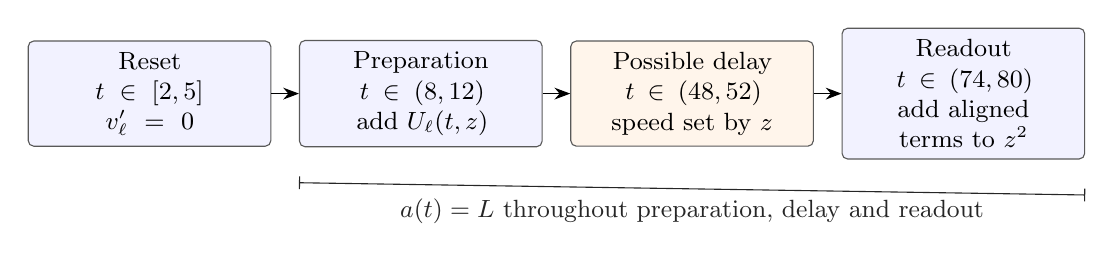
\begin{tikzpicture}[
  phase/.style={draw=black!65,rounded corners=2pt,align=center,
    minimum height=1.25cm,text width=2.8cm,font=\small,inner sep=4pt},
  >={Stealth[length=2mm]}
]
\node[phase,fill=blue!5] (reset) {Reset\\\(t\in[2,5]\)\\\(v'_\ell=0\)};
\node[phase,fill=blue!5,right=0.35cm of reset] (prep)
  {Preparation\\\(t\in(8,12)\)\\add \(U_\ell(t,z)\)};
\node[phase,fill=orange!8,right=0.35cm of prep] (slow)
  {Possible delay\\\(t\in(48,52)\)\\speed set by \(z\)};
\node[phase,fill=blue!5,right=0.35cm of slow] (read)
  {Readout\\\(t\in(74,80)\)\\add aligned terms to \(z^2\)};
\draw[->] (reset)--(prep);
\draw[->] (prep)--(slow);
\draw[->] (slow)--(read);
\draw[|-|,black!85] ([yshift=-0.45cm]prep.south west)
  -- node[below,font=\small,align=center]
  {\(a(t)=L\) throughout preparation, delay and readout}
  ([yshift=-0.45cm]read.south east);
\end{tikzpicture}
\caption{Clock intervals during a complete passage, shown schematically
and not to scale. Values refer to the clock before each update.
All registers reset before preparation. Each channel is read at most
once; for a channel that is read, its preparation signals give a bounded
contribution at that readout.}
\label{fig:clock}
\end{figure}


\subsection{Continuous differentiability}

\begin{proposition}
\label{prop:regularity}
For the choices above, with $q$ finite and $L>\max\{B,2\}$, the series
\eqref{eq:input} defines $C^1$ maps
$U_\ell\colon(\mathbb R/100\mathbb Z)\times\Sigma\to\mathbb C$.
Consequently, \eqref{eq:map} defines a $C^1$ self-map of the nonempty
compact smooth manifold $M$.
\end{proposition}

\begin{proof}
We first estimate the input series in the fixed product Riemannian
metric, then pass to source coordinates.  The chain rule and
$\|DG\|\le B$ give
\begin{equation}
\label{eq:prediction-derivative}
 \|D(G^m)\|\le B^m,\qquad \|DT_m\|\le B^m.
\end{equation}
The second bound uses the real projection $\operatorname{pr}_1$, whose
derivative has norm one everywhere.  In particular, it requires no
choice of output chart for $G^m$.

For an integer $k\ge1$, let
\[
 \Phi_k(z)=\chi(z)(z/|z|)^k\quad(z\in\mathbb C\setminus\{0\}),
 \qquad \Phi_k(0)=\Phi_k(\infty)=0.
\]
These are smooth complex-valued functions.  The support of $\chi$ lies
in a fixed compact annulus, on which the angular map $z\mapsto z/|z|$
and its first derivative are bounded.  The product and chain rules
therefore give a constant $C_\chi$, independent of $k$, such that
\begin{equation}
\label{eq:angular-derivative}
 \|\Phi_k\|_\infty\le1,\qquad
 \|D\Phi_k\|_\infty\le C_\chi(1+k).
\end{equation}
The extensions vanish on fixed neighborhoods of both poles.

Write the $m$th summand, including its prefactor, as
\[
 F_{\ell,m}(t,z)=\frac{L^{1-m}}{10}
             \alpha(t)\beta_\ell(T_m(t,z))\Phi_{2^{m+1}}(z).
\]
Its differential is
\begin{align*}
 DF_{\ell,m}=\frac{L^{1-m}}{10}\bigl(&
 \alpha'(t)\beta_\ell(T_m)\Phi_{2^{m+1}}\,dt\\
 &+\alpha(t)\beta_\ell'(T_m)\Phi_{2^{m+1}}\,DT_m\\
 &+\alpha(t)\beta_\ell(T_m)D\Phi_{2^{m+1}}\bigr).
\end{align*}
Since there are finitely many $\beta_\ell$, their first derivatives have
a common bound.  Equations~\eqref{eq:prediction-derivative}
and~\eqref{eq:angular-derivative} yield a constant $C$, independent of
$\ell$ and $m$, with
\begin{equation}
\label{eq:input-derivative-bound}
 \|F_{\ell,m}\|_\infty+\|DF_{\ell,m}\|_\infty
 \le C L^{1-m}\bigl(1+B^m+2^{m+1}\bigr).
\end{equation}
The prediction and angular derivatives occur in separate product-rule
terms; their bounds are added.  Each of the three resulting geometric
series converges by \eqref{eq:gain-choice}.

For completeness, cover $[0,100]\times\Sigma$ by finitely many relatively
compact source coordinate neighborhoods $V_j$ whose closures lie in larger coordinate
charts $W_j\subset\mathbb R\times\Sigma$.  If $\kappa_j$ is the chart
on $W_j$, the norm of $D\kappa_j^{-1}$ on
$\kappa_j(\overline{V_j})$ is bounded by a constant $C_j$ independent of
$m$.  Thus the coordinate derivatives of
$F_{\ell,m}\circ\kappa_j^{-1}$ satisfy \eqref{eq:input-derivative-bound}
with the additional fixed factor $C_j$.  The series of functions and
of all their first coordinate derivatives consequently converge
uniformly on every such neighborhood.  The usual differentiation
theorem for series now applies: on a smaller coordinate ball, integrate
the first derivatives of the partial sums along line segments and pass
to the uniform limit.  This identifies the derivative of the limit
with the continuous limit of the derivatives.  Hence each $U_\ell$ is
$C^1$ on the fundamental strip.

This proof also covers data with arbitrarily late predicted visits.
At a datum for which $\beta_\ell(T_m)=0$ for every $m$, each summand and
its first derivative vanish: a differentiable nonnegative function has
derivative zero at any zero.  Uniform convergence of the derivative
tails ensures continuity even when nearby nonzero summands have indices
tending to infinity.  No regularity of a selected hitting time is needed.

Because $\alpha$ vanishes near $0$ and $100$, the input and all its
first derivatives vanish on neighborhoods of the periodic seams.
The periodic extension is therefore $C^1$.  Because $\chi$ vanishes
near zero and infinity, the same holds in fixed neighborhoods of the
two poles, so the angular expression introduces no coordinate
singularity.  We also have the uniform bound
\begin{equation}
\label{eq:input-size}
 |U_\ell(t,z)|\le\frac1{10}\sum_{m=1}^{\infty}L^{1-m}
             =\frac{L}{10(L-1)}.
\end{equation}

The clock component of \eqref{eq:map} is smooth and well-defined modulo
$100$.  Each register component is $C^1$ and takes its values in the
fixed disk of radius $3L+L/(10(L-1))$ in the affine chart.  This includes
all source values $v_\ell=\infty$, since $S$ is smooth and zero near
infinity.

It remains to check the main component at $z=\infty$.  Set
\[
 C_0(t,v_1,\ldots,v_q)=20\sum_{\ell=1}^q\bar\beta_\ell(t)S(v_\ell),
 \qquad |C_0|\le60q.
\]
This is a smooth function of all its variables.  In the source inverse
coordinate $w=1/z$ and the corresponding inverse coordinate for the
output, the main component is
\begin{equation}
\label{eq:infinity-chart}
 w'=\frac{w^2}{1+C_0w^2}.
\end{equation}
For $|w|<[2(60q+1)]^{-1/2}$ the denominator has modulus greater than
$1/2$, uniformly in $t$ and the registers.  Formula~\eqref{eq:infinity-chart}
therefore extends smoothly to $w=0$, with value zero.  At all finite
$z$, including $z=0$, the main component is already smooth in the
affine chart.  These checks establish the asserted global $C^1$
regularity of $f$.
\end{proof}

\section{Attraction of every orbit}\label{sec:orbits}

The registers in Section~\ref{sec:construction} have two tasks: they erase
all previous data before each preparation interval, and they supply additions
with the same phase as the main square at each subsequent readout.  We now
prove that these additions force every orbit whose lifted clock is unbounded
to escape to infinity.  A bounded clock instead forces the main coordinate
to zero.

Write $\mathbf v=(v_1,\ldots,v_q)$ and define the compact sets
\begin{equation}\label{eq:attracting-sets}
\begin{split}
 Z_0&=\{(50\bmod100,0,\mathbf v):\mathbf v\in\Sigma^q\},\\
 Z_\infty&=\{(t,\infty,0,\ldots,0):t\in\mathbb R/100\mathbb Z\}.
\end{split}
\end{equation}
Both are forward invariant under~\eqref{eq:map}.  On $Z_0$ one has
$h(50,0)=0$, all readout coefficients and inputs vanish, and the registers
update by $v_\ell\mapsto LS(v_\ell)$.  On $Z_\infty$ the main coordinate stays at
infinity, the clock advances by one, and the zero registers remain zero.

We keep the original time indices throughout the proof.  Thus, for an
arbitrary orbit, write
\[
 f^n(x)=(t_n\bmod100,z_n,v_{n,1},\ldots,v_{n,q}),\qquad
 t_{n+1}=t_n+h(t_n,z_n),
\]
where $t_0\in\mathbb R$ is any lift of the initial clock.  In particular,
\begin{equation}\label{eq:clock-increments}
 0\le t_{n+1}-t_n\le1.
\end{equation}

\begin{proposition}\label{prop:attraction}
For the map $f:M\to M$ constructed in Section~\ref{sec:construction}, every
$x\in M$ satisfies
\[
 \operatorname{dist}\bigl(f^n(x),Z_0\cup Z_\infty\bigr)\longrightarrow0
 \qquad(n\longrightarrow\infty)
\]
in every compatible metric on $M$.
More precisely, if the lifted clock of the orbit is bounded above, then
the clock converges to $50$ modulo $100$ and $z_n\to0$.
If that lift is unbounded above, then $z_n\to\infty$ in $\Sigma$ and all
registers are identically zero from some time onward.
\end{proposition}

\subsection{Bounded clocks and complete passages}

\begin{lemma}\label{lem:bounded-clock}
If $(t_n)$ is bounded above, then $t_n\to50+100k$ for some integer $k$ and
$z_n\to0$.  No condition on the initial register values is required.
\end{lemma}

\begin{proof}
Monotonicity gives a finite limit $t_*$, and hence
$h(t_n,z_n)=t_{n+1}-t_n\to0$.  Since $0\le b(t_n)\le h(t_n,z_n)$,
continuity and the zero set of $b$ imply $t_*=50+100k$.
For all sufficiently large $n$ the clock therefore avoids every readout
support, so $z_{n+1}=z_n^2$.  Moreover, $|z_n|\ge3/4$, including $z_n=\infty$,
would give $e(z_n)=1$ and $h(t_n,z_n)=1$.  Thus eventually $z_n$ is finite
with $|z_n|<3/4$.  Starting at such a time $N$ after all readouts have ceased,
\[
 |z_{N+r}|=|z_N|^{2^r}\longrightarrow0.
\]
The registers may have arbitrary behavior; all their values are included
in the definition of $Z_0$.
\end{proof}

For the rest of the passage analysis, assume $t_n\to+\infty$ and $z_0$ is
finite.  Every $z_n$ is then finite, because the added terms in
\eqref{eq:map} are finite.  Choose an integer $k$ with $100k>t_0$ and set
\[
 N_k=\min\{n\ge0:t_n\ge100k\},\qquad
 N_{k+1}=\min\{n\ge0:t_n\ge100(k+1)\}.
\]
These indices exist.  By~\eqref{eq:clock-increments},
$0\le t_{N_k}-100k<1$.  We call the indices
$N_k\le n<N_{k+1}$ a \emph{complete passage} and, for this fixed passage,
write
\[
 s_n=t_n-100k,\qquad
 I=\{n:N_k\le n<N_{k+1},\ \alpha(s_n)>0\}.
\]
The symbol $s_n$ is a translated clock reading, not a new time index.
Within the passage $0\le s_n<100$, and the periodic coefficients of
\eqref{eq:map} can be evaluated at $s_n$.  In particular,
$\bar\beta_\ell(t_n)=\beta_\ell(s_n)$ there.  Every later period is also a complete
passage because the lift is already assumed unbounded.

\begin{lemma}\label{lem:passage-preparation}
In every complete passage as above, all registers are reset to zero before
the first index in $I$.  The set $I$ is nonempty, has at most five elements,
and contains an index $i$ with $\alpha(s_i)=1$.  For every $i\in I$,
\begin{equation}\label{eq:preparation-radius}
 |z_i|>\tfrac12.
\end{equation}
There also exists an index $j$ in this passage with $s_j\in[76,77]$ and
$\beta_\ell(s_j)=1$ for at least one $\ell$.
\end{lemma}

\begin{proof}
Let $r$ be the first index in the passage with $s_r\ge2$.  The preceding
reading is below $2$, so $2\le s_r<3$.  At time $r$ one has $a(s_r)=0$ and
$\alpha(s_r)=0$, whence $U_\ell(s_r,z_r)=0$ and
\[
 v_{r+1,\ell}=0\qquad(1\le \ell\le q).
\]
This conclusion holds even if any earlier register was at infinity.
Until preparation starts, the inputs remain zero, and $S(0)=0$ keeps all
registers zero.

On $(8,12)$ the clock speed is exactly one.  Its readings in that interval
therefore belong to a single translate of the integers, which gives
$|I|\le5$.  The first reading at least $9$ belongs to $[9,10)$ by
\eqref{eq:clock-increments}; there $\alpha=1$.  Similarly, the first reading
at least $76$ belongs to $[76,77)$, where the plateau-covering property of
the $\beta_\ell$ supplies a coefficient equal to one.  All these crossings
occur in the passage because $s_n$ eventually reaches $100$.

Suppose now that $i\in I$ and $|z_i|\le1/2$.  As long as
$s_n\in[8,50]$ and $|z_n|\le1/2$, there is no readout, $e(z_n)=0$, and
\[
 z_{n+1}=z_n^2,\qquad s_{n+1}=s_n+b(s_n)\le50.
\]
The clock cannot decrease, and $|z_{n+1}|\le1/4\le1/2$.  These two
conditions thus persist by induction from time $i$, keeping $s_n\le50$
forever.  This contradicts the assumed complete passage.  This also
excludes the endpoint $|z_i|=1/2$ and proves~\eqref{eq:preparation-radius}.
\end{proof}

\subsection{Prediction and linearity up to a register's readout}

Fix one complete passage.  The next two lemmas identify the value of a
register at its readout.  The prediction uses the uncontrolled map $G$,
whose main coordinate need not agree with the actual main coordinate after
a readout.  Only their clock coordinates must continue to agree.

\begin{lemma}\label{lem:clock-prediction}
For a given $\ell$, at most one index $j$ in the passage satisfies
$\beta_\ell(s_j)>0$.  If such $j$ exists, then, for every $i\in I$ and every
integer $m\ge1$,
\begin{equation}\label{eq:prediction-single-hit}
 \beta_\ell\bigl(T_m(s_i,z_i)\bigr)=
 \begin{cases}
  \beta_\ell(s_j),&m=j-i,\\
  0,&m\ne j-i.
 \end{cases}
\end{equation}
Here $\beta_\ell$ is the function on $\mathbb R$ used in~\eqref{eq:input},
not its periodization.
\end{lemma}

\begin{proof}
Fix $i\in I$, and let $r_{70}$ and $r_{82}$ be the first indices after $i$
with $s_{r_{70}}\ge70$ and $s_{r_{82}}\ge82$, respectively.  Before
$r_{70}$ all readout coefficients vanish.  The actual pair $(s_n,z_n)$
therefore follows $G$ exactly from time $i$ through time $r_{70}$.
At the latter time $s_{r_{70}}\in[70,71)$.  Throughout $[70,82]$ one has
$b=1$, so both the actual and predicted clock increments are one,
independently of their respective main coordinates.  Starting with the
equal clocks at time $r_{70}$, induction gives
\begin{equation}\label{eq:clock-prediction-agreement}
 T_{n-i}(s_i,z_i)=s_n\qquad(i<n\le r_{82}),
\end{equation}
including after any main-coordinate additions.  The predicted clock is
nondecreasing at all later times.  Once it reaches $82$, it cannot return
to any support of the nonperiodic $\beta_\ell$, all of which lie in $(74,80)$.

The support of a fixed $\beta_\ell$ lies in an interval of length less than
one.  If $\beta_\ell(s_j)>0$, the next clock reading is $s_j+1$, strictly
beyond that support interval.  Monotonicity then rules out any later
positive value of this $\beta_\ell$; the same argument rules out two positive
values in either order.  Equation~\eqref{eq:clock-prediction-agreement}
identifies every possible predicted hit with an actual hit in this
passage, and later predicted hits are impossible.  This proves
\eqref{eq:prediction-single-hit}.
\end{proof}

\begin{lemma}\label{lem:register-linearity}
Let $j$ be an index in the fixed complete passage and let $\ell$ satisfy
$\beta_\ell(s_j)>0$.  Then $|v_{j,\ell}|\le1/2$, $S(v_{j,\ell})=v_{j,\ell}$, and
\begin{equation}\label{eq:register-at-readout}
 v_{j,\ell}=\frac{\beta_\ell(s_j)}{10}
 \sum_{i\in I}\alpha(s_i)\chi(z_i)
 \left(\frac{z_i}{|z_i|}\right)^{2^{j-i+1}}.
\end{equation}
This conclusion does not assume any alignment of the summands' phases.
\end{lemma}

\begin{proof}
Put $i_0=\min I$ and, for each $i\in I$, define
\[
 c_i=\frac{\beta_\ell(s_j)}{10}\alpha(s_i)\chi(z_i)
      \left(\frac{z_i}{|z_i|}\right)^{2^{j-i+1}}.
\]
The phases are defined by~\eqref{eq:preparation-radius}.
Lemma~\ref{lem:clock-prediction} and~\eqref{eq:input} give the exact input
\begin{equation}\label{eq:input-target-time}
 U_\ell(s_i,z_i)=L^{1+i-j}c_i\qquad(i\in I).
\end{equation}
The input at time $i$ first enters $v_{i+1,\ell}$; it receives $j-i-1$
subsequent factors of $L$ before $v_{j,\ell}$ is read.  Thus its coefficient
would be $L^{1+i-j}L^{j-i-1}=1$ if the register remained in the region
where $S$ is the identity.  We verify that region condition directly.

For every integer $u$ with $i_0\le u\le j$, define the candidate value
\[
 w_u=L^{u-j}\sum_{\substack{i\in I\\i<u}}c_i.
\]
The triangle inequality and $|I|\le5$ give
\begin{equation}\label{eq:register-partial-sum-bound}
 |w_u|\le\frac{|I|}{10}L^{u-j}\le\tfrac12.
\end{equation}
By Lemma~\ref{lem:passage-preparation}, $v_{i_0,\ell}=0=w_{i_0}$.
For $i_0\le u<j$ the clock lies between the preparation and readout
intervals, so $a(s_u)=L$.  The input is zero unless $u\in I$, and otherwise
it is $L^{1+u-j}c_u$ by~\eqref{eq:input-target-time}.  Consequently
\[
 w_{u+1}=Lw_u+U_\ell(s_u,z_u).
\]
If $v_{u,\ell}=w_u$, the bound~\eqref{eq:register-partial-sum-bound} implies
$S(v_{u,\ell})=w_u$, so the actual register update gives
$v_{u+1,\ell}=w_{u+1}$.  Induction proves $v_{u,\ell}=w_u$ all the way through
$u=j$.  Every preparation index precedes $j$, hence $w_j=\sum_{i\in I}c_i$,
which proves~\eqref{eq:register-at-readout} and the stated bounds.

This induction concerns only the particular register whose readout is at
$j$.  Another register can already have been read and can subsequently
leave the unit disk.  By Lemma~\ref{lem:clock-prediction}, its readout
coefficient is zero for the rest of this passage.  Registers do not enter
one another's updates, so such later nonlinear behavior has no effect on
the induction just proved.
\end{proof}

\subsection{Phase alignment and escape}

The register values have now been established without any radial or phase
assumption beyond~\eqref{eq:preparation-radius}.  Their phases can therefore
be used to prove the main-coordinate growth.

\begin{lemma}\label{lem:passage-escape}
In a complete passage with finite main coordinate, let $i_0=\min I$.
For every $i_0\le n<N_{k+1}$, $z_n\ne0$ and
\begin{equation}\label{eq:square-lower-bound}
 |z_{n+1}|\ge |z_n|^2,
 \qquad
 \frac{z_{n+1}}{|z_{n+1}|}
   =\left(\frac{z_n}{|z_n|}\right)^2.
\end{equation}
Moreover, some index $N$ with $i_0\le N<N_{k+1}$ satisfies $|z_N|>1$.
\end{lemma}

\begin{proof}
Set $\theta=z_{i_0}/|z_{i_0}|$.  Before the first readout, the main
coordinate squares exactly, so it stays nonzero and its phase at time $n$
is $\theta^{2^{n-i_0}}$.  In particular this holds at every preparation
index $i\in I$, since all preparation precedes all readouts.

Proceed chronologically through the readout indices.  Suppose the phase at
time $j$ is $\theta^{2^{j-i_0}}$ and $z_j\ne0$.  For every $i\in I$ the
phase appearing in~\eqref{eq:register-at-readout} is
\[
 \left(\frac{z_i}{|z_i|}\right)^{2^{j-i+1}}
 =\left(\theta^{2^{i-i_0}}\right)^{2^{j-i+1}}
 =\theta^{2^{j-i_0+1}},
\]
which is the phase of $z_j^2$.  Lemma~\ref{lem:register-linearity} applies
separately to each $\ell$ with $\beta_\ell(s_j)>0$.  The other channels have zero
coefficient in the main update.  Thus that update is exactly
\begin{equation}\label{eq:aligned-main-update}
 z_{j+1}=
 \left(
 |z_j|^2+
 2\sum_{\ell=1}^q\beta_\ell(s_j)^2
       \sum_{i\in I}\alpha(s_i)\chi(z_i)
 \right)\theta^{2^{j-i_0+1}}.
\end{equation}
One factor of $\beta_\ell(s_j)$ comes from the input and the other from the
readout in~\eqref{eq:map}; both are essential to this coefficient.
Every added coefficient is nonnegative, and the baseline $|z_j|^2$ is
strictly positive.  This proves nonvanishing, phase doubling, and the
square lower bound at this readout, even if all its inputs vanish.
Between readouts there is exact squaring.  Induction therefore proves
\eqref{eq:square-lower-bound} through the end of the passage, including
simultaneous readouts of several channels and successive readouts of
different channels.

If some preparation value already has $|z_i|>1$, take $N=i$.  Otherwise
$1/2<|z_i|\le1$ for every $i\in I$.  Choose $i_*$ with
$\alpha(s_{i_*})=1$, supplied by Lemma~\ref{lem:passage-preparation}.
The prescribed cutoff satisfies $\chi(z_{i_*})=1$, including when
$|z_{i_*}|=1$.  The same lemma supplies a readout $j_*$ and a channel $\ell_*$
with $s_{j_*}\in[76,77]$ and $\beta_{\ell_*}(s_{j_*})=1$.
In~\eqref{eq:aligned-main-update}, the single pair $(\ell_*,i_*)$ therefore
adds $2$ to the radius, and all other terms have the same phase.  Hence
\[
 |z_{j_*+1}|\ge |z_{j_*}|^2+2>2.
\]
Taking $N=j_*+1$ proves the claim; this index is still in the passage
because $s_{j_*+1}\le78<100$.
\end{proof}

\begin{proof}[Proof of Proposition~\ref{prop:attraction}]
If the lift is bounded, Lemma~\ref{lem:bounded-clock} proves the asserted
coordinate limits.  In a product metric the distance to $Z_0$ consequently
tends to zero, irrespective of the registers.

If $z_0=\infty$, it remains at infinity, all inputs vanish, and the clock
advances by one at every step.  A translate of the integer lattice meets
the reset interval $[2,5]$ modulo $100$.  At such a step $a=0$, so every
register becomes zero, regardless of its initial value, and stays zero.
The orbit then lies in $Z_\infty$.

It remains to consider an unbounded lift with finite $z_0$.  Choose any
complete passage and an index $N$ with $|z_N|>1$ given by
Lemma~\ref{lem:passage-escape}.  Its square lower bound continues through
the rest of that passage.  We spell out why it also holds at every later
time.  After the current readout region $(74,80)$, all readout multipliers
vanish until the next period's region $(174,180)$ in the same translated
coordinate.  In particular, the main variable squares exactly across the
period boundary and throughout the next reset and preparation intervals.
An old register, however large, cannot alter $z$ there.  It is erased by
the next reset before any new preparation input is entered.

Every later period is a complete passage by the unbounded-lift assumption.
Lemma~\ref{lem:passage-escape} therefore applies afresh from its first
preparation index through its end.  The intervening indices, before that
first preparation, have no readout and give exact squaring.  These intervals
cover every time after $N$, and hence
\begin{equation}\label{eq:escape-growth}
 |z_{N+r}|\ge |z_N|^{2^r}\qquad(r\ge0).
\end{equation}
This argument does not require $\chi$ to vanish immediately after the
radius exceeds one.  New inputs in later periods still have nonnegative
weights $\alpha\chi$, satisfy the register bound, and give the aligned
additions in~\eqref{eq:aligned-main-update}.  Thus they preserve
\eqref{eq:escape-growth} even while $\chi$ remains nonzero.

It follows that $z_n\to\infty$ in $\Sigma$.  Since $\chi$ vanishes in a
neighborhood of infinity, there is a time after which $\chi(z_n)=0$ at
every step.  All inputs $U_\ell(t_n,z_n)$ are then zero.  A later reset, which
exists because the clock lift is unbounded, makes every register zero;
the recurrence and $S(0)=0$ keep them zero forever.  The distance to
$Z_\infty$ therefore tends to zero.

We have proved the assertion in a product metric.  All compatible metrics
on the compact space $M$ are uniformly equivalent, so the same convergence
in distance holds for any such metric.  The conclusion is pointwise in
the initial state; no uniform entry time is asserted.
\end{proof}

\section{Vanishing entropy}\label{sec:entropy}

Proposition~\ref{prop:attraction} gives pointwise attraction to
$Z_0\cup Z_\infty$.  We first prove that such attraction transfers zero
entropy from a compact invariant set to the whole space.  The argument
uses a uniform bound on the proportion of orbit blocks outside a
neighborhood of that set; it requires no uniform eventual-entry time.

The variational principle also yields this conclusion
\cite[Section~3]{Misiurewicz1976}: invariance and bounded convergence
force every invariant probability measure to be supported on the
attracting set. The direct proof below makes the exceptional-block
estimate explicit.

\begin{lemma}[Entropy localization]\label{lemma:localization}
Let $F:X\to X$ be a continuous map of a nonempty compact metric space
$(X,d)$, and let $Z\subseteq X$ be a nonempty compact set with
$F(Z)\subseteq Z$.  Suppose that
\[
  h_{\mathrm{top}}(F|_Z)=0
  \quad\text{and}\quad
  d(F^n x,Z)\longrightarrow 0
  \quad\text{for every }x\in X.
\]
Then $h_{\mathrm{top}}(F)=0$.
\end{lemma}

\begin{proof}
Write $s_X(n,\varepsilon)$ and $s_Z(n,\varepsilon)$ for the separated-set
cardinalities of $F$ and $F|_Z$, respectively.  Fix $\varepsilon>0$ and
an integer $m\geq1$, and define
\[
  d_m(x,y)=\max_{0\leq j<m}d(F^j x,F^j y).
\]
This metric induces the original topology of $X$.  Choose a largest
$(m,\varepsilon/4)$-separated subset of $Z$, of cardinality
$P=P(m)=s_Z(m,\varepsilon/4)$.  Its open $d_m$-balls of radius
$\varepsilon/2$, taken in $X$, have union $V$ containing $Z$: otherwise a
point of $Z$ at $d_m$-distance greater than $\varepsilon/4$ from every
center could be added to the separated set.  Also choose $Q=Q(m)$
open $d_m$-balls of radius $\varepsilon/2$ covering $X$.

We claim that for every $0<\tau<1$ there is an integer $J\geq1$ such
that
\begin{equation}\label{eq:sparse-entropy-blocks}
  \#\{0\leq i<r:F^{mi}x\notin V\}\leq \tau r+J
  \qquad(x\in X,\ r\geq1).
\end{equation}
Indeed, since $Z$ is compact and $V$ is an open neighborhood of $Z$,
the attraction hypothesis implies that $F^{mi}x\in V$ for all
sufficiently large $i$, with the threshold allowed to depend on $x$.
Consequently, for each $x$ there is an integer $k_x\geq1$ for which
\[
  \#\{0\leq i<k_x:F^{mi}x\notin V\}<\tau k_x.
\]
Let $I_x=\{0\leq i<k_x:F^{mi}x\in V\}$.  The open neighborhood
\[
  O_x=\bigcap_{i\in I_x}(F^{mi})^{-1}(V)
\]
of $x$ preserves all these visits: every $y\in O_x$ has fewer than
$\tau k_x$ indices outside $V$ among its first $k_x$ samples.
Choose a finite cover $O_{x_1},\ldots,O_{x_a}$ of $X$, and put
$J=\max_{1\leq b\leq a}k_{x_b}$.

Starting at $x$, choose a member of this cover containing the current
point and follow the corresponding number $k_{x_b}$ of iterates of
$F^m$.  Restart the same procedure at the next point, concatenating
these segments for as long as the selected segment fits within the
first $r$ samples.  The final remainder has length $\ell<J$.
The completed segments contribute at most $\tau(r-\ell)$ samples
outside $V$, and the remainder contributes at most $\ell$.  This
proves~\eqref{eq:sparse-entropy-blocks}, including when no segment
fits.  In particular, this compactness argument bounds a proportion
of exceptional samples without bounding their last occurrence.

Now encode the first $r$ blocks of length $m$ of an orbit.  Record
the subset of indices $i$ for which $F^{mi}x\notin V$.  At every other
index choose one of the $P$ balls covering $V$ that contains
$F^{mi}x$; at an exceptional index choose one of the $Q$ balls
covering $X$.  Choose the first available ball in a fixed ordering
of each cover.  By~\eqref{eq:sparse-entropy-blocks}, the number of
possible descriptions is at most
\begin{equation}\label{eq:entropy-description-count}
  2^r P^r Q^{\tau r+J}.
\end{equation}
Here $2^r$ bounds the number of subsets, and $P,Q\geq1$ allow the
displayed overcount even if $\tau r+J\geq r$.  Two points with the
same description lie in the same radius-$\varepsilon/2$ ball at each
block, so their distance is less than $\varepsilon$ at every time
$0,\ldots,mr-1$.  Thus an $(mr,\varepsilon)$-separated set has at most
the cardinality in~\eqref{eq:entropy-description-count}.

For arbitrary $n$, use $r=\lceil n/m\rceil$ and
$s_X(n,\varepsilon)\leq s_X(mr,\varepsilon)$.  Taking the orbit-length
limit with $m$ and $\tau$ fixed gives
\[
  \limsup_{n\to\infty}\frac{1}{n}\log s_X(n,\varepsilon)
  \leq \frac{\log 2+\log P(m)+\tau\log Q(m)}{m}.
\]
First let $\tau\downarrow0$ with $m$ fixed.  Next let $m\to\infty$.
The hypothesis $h_{\mathrm{top}}(F|_Z)=0$ implies
\[
  \limsup_{m\to\infty}\frac{1}{m}\log P(m)=0,
\]
because every fixed-scale entropy rate is nonnegative and bounded
above by the topological entropy.  The right-hand side therefore
tends to zero.  This holds for every $\varepsilon>0$, proving the lemma.
\end{proof}

It remains to compute the entropy on the invariant sets from
Section~\ref{sec:orbits}.  The register map has a possibly
nonmonotone radial cutoff far from the origin, but its first image
lies in a disk where the radius map is nondecreasing.  The following
lemma includes the initial step on the whole sphere.

\begin{lemma}[Entropy of the register dynamics]\label{lemma:register-entropy}
Let $\Sigma=\mathbb C\cup\{\infty\}$ be the sphere, let $A>0$, and
write $D_A=\{v\in\mathbb C:|v|\leq A\}$.  Suppose that a continuous
map $T:\Sigma\to D_A$ satisfies
\[
  T(re^{i\theta})=R(r)e^{i\theta}
  \qquad(0\leq r\leq A),
\]
where $R:[0,A]\to[0,A]$ is continuous and nondecreasing, with
$R(0)=0$.  Then the coordinatewise map
$T^{\times q}:\Sigma^q\to\Sigma^q$ has zero topological entropy
for every integer $q\geq1$.
\end{lemma}

\begin{proof}
Fix a compatible metric $d_\Sigma$ on $\Sigma$ and use its maximum
product metric on $\Sigma^q$.  Fix $\varepsilon>0$.  Uniform continuity
of the polar map
\[
  [0,A]\times\mathbb S^1\longrightarrow D_A,
  \qquad(r,u)\longmapsto ru,
\]
allows a partition of $[0,A]$ into $H$ sufficiently short ordered
intervals and a partition of $\mathbb S^1$ into $K$ sufficiently
short arcs, such that two points have $d_\Sigma$-distance less than
$\varepsilon$ whenever their radii lie in the same interval and their
angular coordinates lie in the same arc.
Use half-open intervals and arcs, with endpoints assigned once,
so that the labels are single-valued.  Let
$b:[0,A]\to\{1,\ldots,H\}$ be the resulting nondecreasing radius
label.

For a radius $r\in[0,A]$ and an integer $N\geq1$, consider its
label vector
\[
  \bigl(b(r),b(R(r)),\ldots,b(R^{N-1}(r))\bigr).
\]
Every coordinate of this vector is nondecreasing as a function of
the initial radius $r$.  Its distinct values therefore form a chain
in the coordinatewise order on $\{1,\ldots,H\}^N$.  Along such a
chain the sum of the coordinates strictly increases whenever the
vector changes, and this sum lies between $N$ and $NH$.  Hence there
are at most
\begin{equation}\label{eq:radius-itinerary-count}
  1+N(H-1)
\end{equation}
radius itineraries.  This orders itineraries by their initial
radii; no monotonicity in time is being asserted.

Each point $v\in D_A$ can be written $v=ru$ with $u\in\mathbb S^1$;
choose $u=1$ when $v=0$.  Its iterates have the representations
$T^jv=R^j(r)u$ with that same $u$, including after a radius becomes
zero.  Thus one angular label, together with the radius itinerary,
gives at most $K[1+N(H-1)]$ descriptions of length-$N$ orbits in
$D_A$.  Points with the same description stay within
$\varepsilon$ throughout those $N$ iterates.

Finally cover the whole compact space $\Sigma^q$ by $C$ sets of
diameter less than $\varepsilon$, and assign each initial point one
cover label.  For $n\geq2$, encode time zero by this label and
encode each coordinate of its first image in $D_A^q$ for the
remaining $N=n-1$ times by the preceding construction.  Points
sharing a complete description stay within $\varepsilon$ in the
maximum product metric for all $n$ times.  Consequently
\begin{equation}\label{eq:register-separated-count}
  s_{\Sigma^q}(n,\varepsilon)
  \leq C\bigl\{K[1+(n-1)(H-1)]\bigr\}^{q}.
\end{equation}
The finite initial cover accounts for all preimages of the disk,
including $\infty$.  The bound grows polynomially in $n$, so its
exponential rate is zero at every $\varepsilon>0$.
\end{proof}

\begin{proposition}\label{prop:zero-entropy}
The map $f$ defined in~\eqref{eq:map} has
$h_{\mathrm{top}}(f)=0$.
\end{proposition}

\begin{proof}
Recall the compact forward-invariant sets of
Proposition~\ref{prop:attraction}:
\[
  \begin{aligned}
    Z_0&=\{(t,z,v_1,\ldots,v_q):t=50\pmod{100},\ z=0\},\\
    Z_\infty&=\{(t,z,v_1,\ldots,v_q):z=\infty,\ v_1=\cdots=v_q=0\}.
  \end{aligned}
\]
On $Z_0$, the clock and main coordinate are fixed and the registers
evolve independently by $T(v)=LS(v)$.  By the choice of $S$ in
Section~\ref{sec:construction}, $T(\Sigma)\subseteq D_{3L}$, and on
that disk its radius map is
\[
  R(r)=Lp(r),\qquad 0\leq r\leq 3L.
\]
This map is continuous, nondecreasing, fixes zero, and takes values
in $[0,3L]$.  Lemma~\ref{lemma:register-entropy} therefore gives
$h_{\mathrm{top}}(f|_{Z_0})=0$.

On $Z_\infty$ the only evolving coordinate is the clock, which
advances by $1$ modulo $100$.  Thus $(f|_{Z_\infty})^{100}$ is the
identity.  For $n\geq100$ the orbit metric $d_n$ on this set equals
$d_{100}$, so its separated-set cardinalities are bounded
independently of $n$ at every fixed scale.  In particular,
$h_{\mathrm{top}}(f|_{Z_\infty})=0$.

For $Z=Z_0\cup Z_\infty$, splitting a separated set between these
two invariant subsets gives
\[
  s_Z(n,\varepsilon)\leq
  s_{Z_0}(n,\varepsilon)+s_{Z_\infty}(n,\varepsilon).
\]
Both terms have zero exponential rate, hence
$h_{\mathrm{top}}(f|_Z)=0$.  Proposition~\ref{prop:attraction}
states that every orbit of $f$ approaches this exact set $Z$.
Lemma~\ref{lemma:localization} now proves
$h_{\mathrm{top}}(f)=0$.
\end{proof}

\section{The homological eigenvalue}\label{sec:homology}

The main coordinate of \(f\) is a bounded additive perturbation of
squaring. Fading out that perturbation gives the homological information
needed for Theorem~\ref{thm:main}.

\begin{proposition}\label{prop:homology}
For the map \(f\) in \eqref{eq:map}, the action
\(f_*:H_2(M;\R)\to H_2(M;\R)\) has eigenvalue \(2\).
\end{proposition}

\begin{proof}
Let \(\pi:M\to\Sigma\) be projection to \(z\), and put \(g(z)=z^2\),
with \(g(\infty)=\infty\). Define
\[
 C(t,v)=20\sum_{\ell=1}^q\bar\beta_\ell(t)S(v_\ell).
\]
Since \(|S|\le3\), we have \(|C|\le60q\). For \(0\le s\le1\), set
\[
 H_s(t,z,v)=z^2+sC(t,v)
\]
when \(z\) is finite, and \(H_s(t,\infty,v)=\infty\).
This is a continuous homotopy from \(g\pi\) to \(\pi f\).
Indeed, in the inverse coordinate \(w=1/z\) at infinity, the output
has inverse coordinate
\[
 \frac{w^2}{1+sC(t,v)w^2}.
\]
For all \(s,t,v\), the denominator is nonzero on one fixed
neighborhood of \(w=0\), since \(|sC|\le60q\).
This verifies continuity jointly in every variable, including \(s\).

By homotopy invariance and functoriality of singular homology
\cite[Theorem~2.10]{Hatcher2002},
\begin{equation}\label{eq:intertwining}
 \pi_*f_*=g_*\pi_*
 \quad\text{on }H_2(M;\R).
\end{equation}
The oriented sphere has \(H_2(\Sigma;\R)\cong\R\), and the action
of \(g\) on this group is multiplication by its degree.
The regular value \(1\) has the two preimages \(1\) and \(-1\).
At either preimage the derivative is complex multiplication by
\(2z\), with positive real determinant \(|2z|^2=4\).
Both local degrees are \(+1\), so \(\deg g=2\)
\cite[Proposition~2.30 and Lemma~2.49]{Hatcher2002}.

The projection \(\pi\) has a section obtained by fixing the clock
and all register coordinates. Therefore
\(\pi_*:H_2(M;\R)\to H_2(\Sigma;\R)\) is surjective.
Write \(A=f_*|_{H_2(M;\R)}\) and \(P=\pi_*\). Equation
\eqref{eq:intertwining} gives \(P(A-2I)=0\), with \(P\ne0\).
If \(A-2I\) were invertible, this equality would imply \(P=0\).
Thus \(2\) is an eigenvalue of \(A\).
\end{proof}

\begin{proof}[Proof of Theorem~\ref{thm:main}]
Proposition~\ref{prop:regularity} constructs a \(C^1\) self-map of
the stated compact smooth manifold.
Proposition~\ref{prop:zero-entropy} gives \(\htop(f)=0\), and
Proposition~\ref{prop:homology} supplies the eigenvalue \(2\) on
\(H_2(M;\R)\). This group is an invariant summand of \(H_*(M;\R)\),
so \(\rho(f_*)\ge2\). Finally, \(S\) vanishes on a neighborhood
of infinity. Holding all other coordinates fixed and varying
one register within that neighborhood leaves every output in
\eqref{eq:map} unchanged. Hence \(f\) is noninvertible.
\end{proof}


\bibliographystyle{plain}
\phantomsection
\addcontentsline{toc}{section}{References}
\bibliography{references}
\end{document}
